Figure.~\ref{fig:sigOverview} provides an overview of the signals and protocols used in the system. 
The aircraft communicates with the cockpit unit using MIL-STD-1553-B. 
The same standard is used between the cockpit unit and the missile warning system (MWS).

\begin{figure}[h]
	\centering
	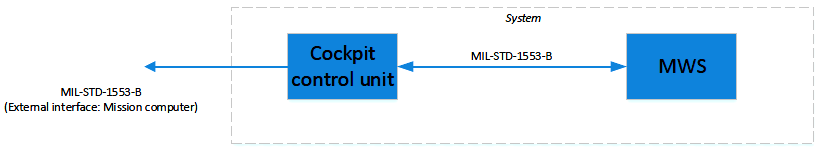
\includegraphics[scale=0.55]{./images/signalOverview.png}\\
	\caption{System signal overview}
    \label{fig:sigOverview}
\end{figure}

Figure.~\ref{fig:hieraOverview} provides an overview of the components comprising the system.
The system has two major parts; the cockpit unit and the pod. 
The pod contains the MWS and components for handling and dispensing the payload.

\begin{figure}[h]
	\centering
	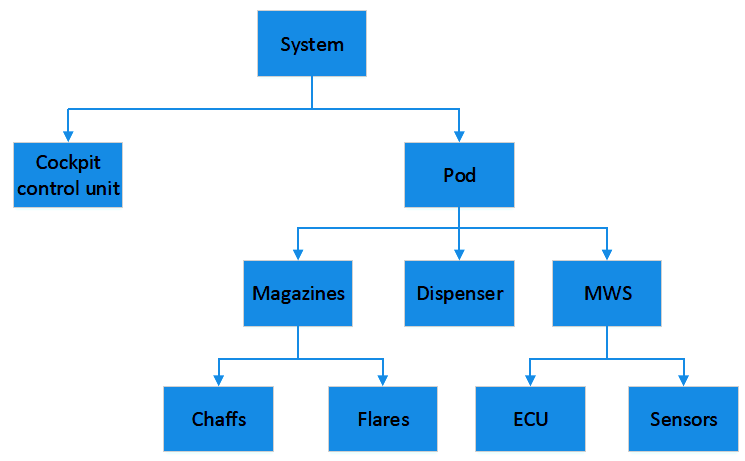
\includegraphics[scale=0.6]{./images/hierarchical.png}\\
	\caption{Hierarchical overview of system}
    \label{fig:hieraOverview}
\end{figure}

